\documentclass{vldb}


\usepackage{enumitem}
\usepackage{framed}
%\usepackage[11pt]{moresize}
\usepackage{cprotect}
\usepackage{enumitem}
\usepackage{listings}
\usepackage{amstext}
\usepackage{amstext}
\usepackage{pdfpages}
\usepackage{alltt}
\usepackage{epstopdf}
\usepackage{xspace,colortbl}
\usepackage[USenglish]{babel}
\usepackage{multirow}
\usepackage[hyphens]{url}
\usepackage{subfigure}
\usepackage{graphicx}%%
\usepackage{amssymb}
\usepackage{fmtcount}
\usepackage{amsfonts}
\usepackage{xspace}
\usepackage{amsmath}
\usepackage{multirow}
\usepackage[mathscr]{eucal}
%\usepackage{psfrag}
\usepackage{colortbl}

\usepackage{amsmath,amssymb}
\usepackage[linesnumbered, ruled,vlined]{algorithm2e}

\usepackage{caption}
\usepackage{graphicx}

\usepackage{bm}
\usepackage[nospace]{cite}
\usepackage{csquotes}
\usepackage{enumitem}
\usepackage{charter}

\usepackage{courier}

\lstset{basicstyle=\ttfamily,breaklines=true}
\lstset{framextopmargin=50pt}

\usepackage{cleveref}

\usepackage{balance}

%\linespread{0.99}

\makeatletter
\def\@copyrightspace{\relax}
\makeatother


\DeclareMathOperator*{\argmin}{arg\,min}
\DeclareMathOperator*{\argmax}{arg\,max}
\newcommand*{\QEDB}{\ensuremath{\square}}%

\newcommand{\sys}{\textsf{DQ}\xspace}


\begin{document}


\newtheorem{theorem}{Theorem}
\newtheorem{example}{Example}
\newtheorem{definition}{Definition}
\newtheorem{problem}{Problem}
\newtheorem{property}{Property}
\newtheorem{proposition}{Proposition}
\newtheorem{lemma}{Lemma}
\newtheorem{corollary}{Corollary}

\newcommand{\detectlib}{\texttt{IsoDetect}\xspace}
\newcommand{\company}{\texttt{Company X}\xspace}
\newcommand{\cond}{\textrm{pred}\xspace}
\newcommand{\dataset}{data set\xspace}
\newcommand{\datasets}{data sets\xspace}
\newcommand{\spview}{\textsf{SPView}\xspace}
\newcommand{\fjview}{\textsf{FJView}\xspace}
\newcommand{\aggview}{\textsf{AggView}\xspace}
\newcommand{\hashfunc}[1]{\textsf{hash}(#1)\xspace}
\newcommand{\hashop}{\textsf{hash}\xspace}
\newcommand{\nsc}{\textsf{NormalizedSC}\xspace}
\newcommand{\rsc}{\textsf{RawSC}\xspace}

\newcommand{\avgfunc}{\ensuremath{\texttt{avg} }\xspace}
\newcommand{\maxfunc}{\ensuremath{\texttt{max} }\xspace}
\newcommand{\minfunc}{\ensuremath{\texttt{min} }\xspace}
\newcommand{\histfunc}{\ensuremath{\texttt{histogram\_numeric} }\xspace}
\newcommand{\countfunc}{\ensuremath{\texttt{count}}\xspace}
\newcommand{\sumfunc}{\ensuremath{\texttt{sum} }\xspace}
\newcommand{\varfunc}{\ensuremath{\texttt{var} }\xspace}
\newcommand{\stdfunc}{\ensuremath{\texttt{std} }\xspace}
\newcommand{\covfunc}{\ensuremath{\texttt{cov} }\xspace}
\newcommand{\corrfunc}{\ensuremath{\texttt{corr} }\xspace}
\newcommand{\medfunc}{\ensuremath{\texttt{median} }\xspace}
\newcommand{\percfunc}{\ensuremath{\texttt{percentile} }\xspace}
\newcommand{\havingfunc}{\ensuremath{\texttt{HAVING} }\xspace}
\newcommand{\selectfunc}{\ensuremath{\texttt{select} }\xspace}
\newcommand{\ratio}{\ensuremath{\rho }\xspace}


\newcommand{\insertion}{\ensuremath{\texttt{INSERT} }\xspace}
\newcommand{\update}{\ensuremath{\texttt{UPDATE} }\xspace}
\newcommand{\delete}{\ensuremath{\texttt{DELETE} }\xspace}

\newcommand{\sysfull}{AlphaClean\xspace}
\newcommand{\sys}{AlphaClean\xspace}
\newcommand{\sysnospace}{AlphaClean}


\newcommand{\tbl}[1]{\textsf{#1}\xspace}
\newcommand{\field}[1]{\textsf{#1}\xspace}
\newcommand{\cost}{\textrm{cost}\xspace}
\newcommand{\ans}{\textsf{ans}\xspace}
\newcommand{\dans}{\Delta\textsf{ans}\xspace}
\newcommand{\cqp}{correction query processing\xspace}
\newcommand{\Cqp}{Correction query processing\xspace}

\newcommand{\reminder}[1]{{{\textcolor{magenta}{\{\{\bf #1\}\}}}\xspace}}
\newcommand{\ewu}[1]{{{\textcolor{blue}{\{\{\bf ewu:\} #1\}}}\xspace}}
\newcommand{\mps}[1]{{{\textcolor{red}{\{\{\bf meelap:\} #1\}}}\xspace}}
\newcommand{\stitle}[1]{\smallskip\noindent\textbf{#1: }}
\newcommand{\ititle}[1]{\smallskip\noindent\textit{#1: }}
\newcommand{\btitle}[1]{\smallskip\noindent\textbf{#1}}


\definecolor{light-gray}{gray}{0.95}
\definecolor{mid-gray}{gray}{0.85}
\definecolor{green}{RGB}{0,176,80}
\definecolor{darkred}{rgb}{0.7,0.25,0.25}
\definecolor{darkgreen}{rgb}{0.15,0.55,0.15}
\definecolor{darkblue}{rgb}{0.1,0.1,0.5}
\definecolor{orange}{RGB}{237,125,49}
\definecolor{blue}{RGB}{68,114,196}
\definecolor{pop}{RGB}{0,21,245}

\newcommand{\white}[1]{{\textcolor{white}{#1}\xspace}}
\newcommand{\blue}[1]{{\textcolor{blue}{{\bf #1}}\xspace}}
\newcommand{\orange}[1]{{\textcolor{orange}{{\bf #1}}\xspace}}
\newcommand{\pop}[1]{{\textcolor{pop}{{\textit{\textbf{#1}}}}\xspace}}
\newcommand{\red}[1]{\textcolor{red}{#1}}
\newcommand{\green}[1]{\textcolor{green}{#1}}
\newcommand{\gray}[1]{\textcolor{light-gray}{#1}}




\newcommand{\specialcell}[2][c]{%
  \begin{tabular}[#1]{@{}c@{}}#2\end{tabular}}

\def\ojoin{\setbox0=\hbox{$\bowtie$}%
  \rule[-.02ex]{.25em}{.4pt}\llap{\rule[\ht0]{.25em}{.4pt}}}
\def\leftouterjoin{\mathbin{\ojoin\mkern-5.8mu\bowtie}}
\def\rightouterjoin{\mathbin{\bowtie\mkern-5.8mu\ojoin}}
\def\fullouterjoin{\mathbin{\ojoin\mkern-5.8mu\bowtie\mkern-5.8mu\ojoin}}

%\setlength{\belowcaptionskip}{-10pt}

%\newcommand{\reminder}[1] {}
\pagestyle{plain}

%\input{coverletter.tex}

%\title{\sys: Declarative Data Cleaning with \\ Learning and Tree-Search}
% \title{\sys: Automatic Data Cleaning For Humans}
% \title{\sys: Automatic Data Cleaning as Planning}
% \title{\sys: Automatic Data Cleaning as Optimization}
%\title{\sys: A Declarative Data Cleaning System Inspired By AlphaGo}
\title{Learning Join Optimization With Deep Reinforcement Learning}

\numberofauthors{1}
\author{ Sanjay Krishnan, Zongheng Yang, Ion Stoica, Joseph Hellerstein, Ken Goldberg  \\
\affaddr{RISELab UC Berkeley} \\
\affaddr{ \{sanjaykrishnan, zongheng, istocia, jmh, goldberg\}@berkeley.edu}\\
\affaddr{}
}

\maketitle

\begin{abstract}
Exhaustive enumeration of all possible join orders is prohibitive for large queries and most query optimizers leverage pruning heuristics (e.g., considering only left-deep plans) and/or optimization heuristics (e.g., cost linearization). 
However, no single technique dominates; the same workload with different cost models can lead to very different results.
Recent work in deep reinforcement learning (Deep RL) may provide an unexpected perspective on this problem. 
Deep RL is a form of approximate dynamic programming and can allow cost-based join order optimizers to efficiently learn between planning instances. 
In essence, the algorithm leverages data to learn how to prune the search space.
We present the \sys optimizer, which currently optimizes SPJ blocks, and evaluate it on the Join Order Benchmark. 
Results suggest \textbf{TODO summarize}
\end{abstract}


%\pagenumbering{gobble}


\section{Introduction}\label{intro}\sloppy
Since most relational database management systems support only dyadic join operators (joining two tables), an algorithm to choose the ``best'' sequence of two-way joins to achieve a k-way join is a core primitive in almost every query optimizer.
Exhaustive enumeration of all possible join orders is prohibitive for large queries.
Due to new visualization and business intelligence tools that automatically generate queries, the prevalence of increasingly large join queries has sparked a renewed interest to effectively scale up join ordering algorithms~\cite{neumann2018adaptive}. 

In practice, query optimizers leverage a combination of pruning heuristics and/or optimization heuristics to make the search for a good plan efficient.
For example, the classical Selinger optimizer restricts its search to left-deep orders~\cite{selinger1979access}.
Left-deep orders still allow for effective index utilization as the intermediate results can be streamed through each index lookup. 
This heuristic is not universally effective, and, in some database architectures, exactly the opposite heuristic is required (i.e., right-deep plans)~\cite{gerber1986data}.
Similarly, there are countless other techniques that exploit other special problem settings, intelligently combine heuristics, or approximate the cost function~\cite{swami1993polynomial,steinbrunn1997heuristic,galindo2008optimizing,ziane1993parallel}. 
For some of methods, precise conditions for optimality are known~(e.g., IK-KBZ~\cite{krishnamurthy1986optimization}). However, for others, given a particular cost function, database, and query workload, it can be very unclear whether the heuristic applies. 

This is not simply an academic concern, and it can be experimentally shown on existing join optimization benchmarks.
Figure \ref{teaser} illustrates this point on a query from the Join Order Benchmark~\cite{leis2015good}, which bases its dataset and queries from the International Movie Database (IMDB). We implemented two different cost models, one similar to~\cite{leis2015good} with a hash-join cost that is linear in the size of the input relations, and one that is similar to the cost models discussed in~\cite{ziane1993parallel} that allows for reuse of already built hash tables.
We use a left-deep dynamic program and a right-deep dynamic program to optimize the joins in the query.
In the first cost model, the best left-deep plan has a 39x lower cost than the best right-deep plan. While in the second cost model, the best right-deep plan has an 8x lower cost than the best left-deep one.
This illustrates that practically, the search problem is unforgiving, where a poor heuristic may suffer orders of magnitudes of optimality.

\begin{figure}
    \centering
    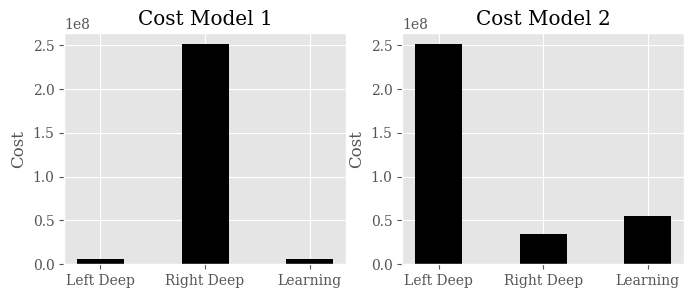
\includegraphics[width=\columnwidth]{figs/teaser.png}
    \caption{\small Query 12b from the Join Order Benchmark with 2 different cost models. Cost model 1 models a hash-join operator with a linear cost in the size of the input relations, and Cost model 2 models re-use of already built hash tables. A learning-based strategy is competitive with the dominant heuristic in both models. \label{teaser}}
\end{figure}

In these dynamic programs, the optimizer incrementally builds optimal joins on subsets of relations.
Leveraging the principle of optimality, it memoizes the optimal join order up-to the current intermediate results.
For a static database, suppose one could hypothetically store all the memoization tables created for all planning instances.
If we had this hypothetical scenario, as the optimizer plans for more queries there is increasing re-use as all possible subplans are covered.
Once this table is fully populated, join ordering would reduce to a hash-table lookup.
In practice, this table would be impossible to fully populate and store.

What if one could represent all of that information with a parametrized statistical model? To do so, we can take inspiration from the Artificial Intelligence field of reinforcement learning (RL)~\cite{sutton1998reinforcement}. RL algorithms use sampling and statistical machine learning to efficiently estimate the long-term benefit of certain decisions.
In our context, this means approximate the query optimizer's cost-to-go function, or what is the long-term value of making a particular join. 
Since the cost-to-go function can be very complex, we sufficiently rich class of functions, like neural networks, to model it.
This is exactly an instance of a Deep RL  algorithm, called Deep Q Networks (DQN), similar to the ones used to play Atari Games or the game of Go.
Going back to Figure \ref{teaser}, we train an RL model on 80 randomly selected queries from the Join Order benchmark and use the learned model to optimize the same query. We find that it is competitive on both cost models.

While the efficacy of machine learning in database internals is still the subject of significant debate~\cite{btree, kraska2018case, mitzenmacher2018model}, we believe that learning strategies for join ordering is a natural fit due to the orders of magnitude of performance at stake. 
This learning based approach gives us flexibility in designing new intelligent enumeration strategies by manipulating how the neural network is trained and how it represents the subplans.
For example, the neural network allows us to efficiently share query processing information across planning instances with the neural network parameters and learn from previously executed queries.
The consequence is enumeration strategies tuned to the specific workload and data.
We can also vary the features used to represent the subplans, to allow the network to capture different properties physical operator selection and selectivities.
We can also train the neural network with observations of actual query execution times and make it robust to faulty cost models.

In short, Deep RL provides a new algorithmic perspective for thinking about join enumeration. 
The essence is to shift the cost of heuristic design to data collection and featurization.
Our system, called \sys, is built on Apache Calcite and we present extensive results on the join order benchmark.
We show \sys optimizes plans well across many different cost models for a relatively modest set of training queries.
Admittedly, this raises a new set of problems including overfitting and avoiding high-variance plans.
We hope that \sys is a first step in an entire spectrum of techniques between pure Deep RL and classical query optimization.


 


\section{Background}
First, we will introduce the algorithmic connection between Reinforcement Learning and the join optimization problem.

\subsection{Query Model}
Consider the following query model.
Let $\{R_1,...,R_T\}$ define a set of relations, and let $\mathcal{R} = R_1 \times ... \times R_T$ denote the cartesian product.
We define an inner join query $q$ as a subset of $q \subseteq \mathcal{R}$ as defined by a conjunctive predicate $\rho_1 \wedge ... \wedge \rho_j$ where each expression $\rho$ is binary boolean function of the attributes of two relations in the set $\rho = R_i.a \{=,!=,>,<\} R_j.b)$. We assume that the number of conjunctive expressions is capped at some fixed size $\mathcal{N}$.
We further assume that the join operation is commutative, left associative, and right associative.
Extending our work to consider left and right outer joins is very straight-forward but we will defer that to that to future work.

We will use the following database of three relations denoting employee salries as a running example throughout the paper:
\[
\text{Emp}(id, name, rank)
\]
\[
\text{Pos}(rank, title, code)
\]
\[
\text{Sal}(code, amount)
\]
Consider the following join query:
\begin{lstlisting}
SELECT *
 FROM Emp, Pos, Sal
 WHERE Emp.rank = Pos.rank AND
 Pos.code = Sal.code
\end{lstlisting}
In this schema, $\mathcal{R}$ denotes the set of tuples $\{(e \in Emp, p \in Pos, s \in Sal)\}$. There are two predicates $\rho_1 = Emp.rank = Pos.rank$ and $\rho_2 = Pos.code = Sal.code$, combined with a conjunction. 
One has several possible options on how to execute that query. For example, one could execute the query as $Emp \bowtie (Sal \bowtie Pos)$. Or, one could execute the query as $Sal \bowtie (Emp \bowtie Pos)$. 

\subsection{Graph Model of Enumeration}
Enumerating the set of all possible dyadic join plans can be expressed as operations on a graph representing the join relationships requested by a query.

\begin{definition}[Query Graph]
Let $G$ define an undirected graph called the \emph{query graph}, where each relation $R$ is a vertex and each $\rho$ defines an edge between vertices. The number of connected components of $G$ are denoted by $\kappa_G$.
\end{definition}

Each possible dyadic join is equivalent to a combinatorial operation called a graph contraction.

\begin{definition}[Contraction]
Let $G = (V,E)$ be a query graph with V defining the set of relations and E defining the edges from the join predicates. A contraction $c$ is a function of the graph parametrized by a tuple of vertices $c=(v_i, v_j)$. Applying $c$ to the graph $G$ defines a new graph with the following properties: (1) $v_i$ and $v_j$ are removed from $V$, (2) a new vertex $v_{ij}$ is added to $V$, and (3) the edges of $v_{ij}$ are the union of the edges incident to $v_i$ and $v_j$. 
\end{definition}

Each contraction reduces the number of vertices by $1$. And, that every feasible dyadic join plan can be described as a sequence of such contractions $c_1 \circ c_2 ...\circ c_{T}$ until $|V| = \kappa_G$. Going back to our running example, suppose we start with a query graph consisting of the vertices $(Emp, Pos, Sal)$. Let the first contraction be $c_1 = (Emp, Pos)$, this leads to a query graph where the new vertices are $(Emp+Pos, Sal)$. Applying the only remaining possible contraction, we arrive at a single remaining vertex $Sal+(Emp+Pos)$ corresponding to the join plan $Sal \bowtie (Emp \bowtie Pos)$. 

The join optimization is to find the best possible one of these contraction sequences. Assume that we have access to a cost model $J$, which is a function that can estimate the incremental cost of a particular contraction $J(c) \mapsto \mathbb{R}_+$. 

\begin{problem}[Join Optimization Problem]
Let $G$ define a query graph and $J$ define a cost model. Find a sequence of $c_1 \circ c_2 ...\circ c_{T}$ terminating in $|V| = \kappa_G$ to minimize:
\[
\min_{c_1,...,c_T} \sum_{i=1}^T J(c_i)
\]\label{joinopt}
\end{problem}

Note how the ``Principle of Optimality'' arises in Problem \ref{joinopt}. Applying each contraction generates a subproblem of a smaller size (a query graph with one less vertex). Each of these subproblems must be solved optimally in any optimal solution. Also note that this model can capture physical operator selection as well. The set of allowed contractions can be typed with an eligible join type e.g., $c=(v_i, v_j, \text{hash})$ or $c=(v_i, v_j, \text{index})$.

\subsection{Greedy vs. Optimal}
A \emph{greedy} solution to this problem is to optimize each $c_i$ independently. The algorithm proceeds as follows: (1) start with the query graph, (2) find the lowest cost contraction, (3) update the query graph and repeat until only one vertex is left. The greedy algorithm, of course, does not consider how local decision might affect future costs. Consider our running example query with the following costs (assume symmetry):
\[J(EP)= 100,~J(SP)= 90,~J((EP)S)= 10,~J((SP)E)= 50\]
The greedy solution would result in a cost of 140 (because it neglects the future effects of a decision), while the optimal solution has a cost of 110.
However, there is an upside, this greedy algorithm has a computational complexity of $O(|V|^3)$---despite the super-exponential search space.

The decision at each index needs to consider the long-term value of its actions where one might have to sacrifice a short term benefit for a long term payoff.
Consider the following way of expressing the optimization problem in the problem statement for a particular query graph $G$:
\begin{equation}
V(G) = \min_{c_1,...,c_T} \sum_{i=1}^T J(c_i)
\label{eq:main}
\end{equation}

We can concisely describe Equation \ref{eq:main} as the function $V(G)$, i.e., given the initial graph $G$, what is the value of acting optimally till the end of the decision horizon. This function is conveniently named the \emph{value function}. Bellman's ``Principle of Optimality'' noted that optimal behavior over an entire decision horizon implies optimal behavior from any starting index $t>1$ as well, which is the basis for the idea of dynamic programming.
So, $V(G)$ can be then defined recursively for any subsequent graph $G'$ generated by future contractions:
\begin{equation}
V(G) = \min_{c}\{~J(c) + \gamma \cdot V(G') ~\}
\label{eq:value}
\end{equation}
Usually, write this value recursion in the following form:
\[
Q(G,c) = J(c) + \gamma \cdot V(G')
\]
Leading to the following recursive definition of the Q-Function (or cost-to-go function):
\begin{equation}
Q(G,c) = J(c) + \gamma \cdot \min_{c'} Q( G',c')
\label{eq:q}
\end{equation}

The Q-Function describes the long-term value of each contraction. 
That means at each $G'$ local optimization of $\min_{c'} Q(G',c')$ is sufficient to derive an optimal sequence of decisions. Put another way, the Q-function is a hypothetical cost function on which greedy descent is optimal and equivalent to solving the original problem.
If we revisit the greedy algorithm, and revise it as follows: (1) start with the query graph, (2) find the lowest \textbf{Q-value} contraction, (3) update the query graph and repeat. This algorithm has a computational complexity of $O(|V|^3)$ (just like the greedy algorithm) but is provably optimal. 

The Q-function is implicitly stored as a table in classical dynamic programming approaches, such as the System R enumeration algorithm. In the System R algorithm, there is a hash table that maps sets of joined relations to their lowest-cost access path:
\begin{lstlisting}
HashMap<Set<Relation>, (Plan, Long)> bestJoins;
\end{lstlisting}
As the algorithm enumerates more subplans, if a particular relation set exists in the table it replaces the access path if the enumerated plan has a lower cost than one in the table. We could equivalently write a different hash table that moves around the elements on the table described above. Instead of a set of relations mapping to a plan and a cost, we could consider a set of relations \emph{and} a plan mapping to a cost: 
\begin{lstlisting}
HashMap<(Set<Relation>, Plan), Long> bestQJoins;
\end{lstlisting}
As the algorithm enumerates more plans, the algorithm put enumerated plans into the table. However, the replacement policy for this table is slightly different than in the classical model. As we enumerate plans, we replace all child plans with the \emph{cost of the parent} if lower. Once this table is constructed, backtracking can be used to retrieve an optimal plan.

\subsection{Learning the Q-Function}
This change would be less efficient implementation in classical dynamic programming, but it crucially allows us to setup a machine learning problem. 
What if we could regress from features of \texttt{(Set<Relation>, Plan)} to a cost based on a small number of observations?
Instead of a Q-Function as a table, it is parametrized as a model:
\[
Q_\theta(f_G,f_c) \approx Q(G,c)
\]
where $f_G$ is a feature vector representing the query graph and $f_c$ is a feature vector representing the particular contraction on the graph. $\theta$ defines the neural network parameters that represent this function. 

The basic strategy to generate observational data, that is, real executions of join plans, and optimize $\theta$ to best explain the observations. Such an optimization problem is a key motivation of a general class of algorithms called Reinforcement Learning~\cite{sutton1998reinforcement}, where statistical machine learning techniques are used to approximate optimal behavior while observing substantially less data that full enumeration. 

For those familiar with the AI literature, this problem defines a Markov Decision Process. $G$ is exactly a representation of the \textbf{state} and $c$ is a representation of the \textbf{action}.
The utility function (or reward) of this process is the negative overall runtime.
The objective of the planning problem is to find a policy, which is a map from a query graph to the best possible join $c$.

In the popular Q-Learning approach~\cite{sutton1998reinforcement}, the algorithm enumerates random samples of decision sequences containing $(G,c, runtime, G')$ tuples forming a trajectory. From these tuples, one can calculate the following value:
\[
y_i = runtime + \arg \max_{u} Q_\theta(G',c)
\]
Each of the $y_i$ can be used to define a loss function since if $Q$ were the true Q function, then the following recurrence would hold:
\[
Q(G,c) = runtime + \arg \max_{u} Q_\theta(G',c)
\]
So, Q-Learning defines a loss:
\[
L(Q) = \sum_{i} \|y_i - Q_\theta(G',c)\|_2^2
\]
This loss can be optimized with gradient descent.
This algorithm is called the Deep Q Network algorithm~\cite{mnih2015human} and was used to learn how to autonomously play Atari Games.
The key implication is that the neural network allows for some ability for the optimizer to extroplate the cost-to-go even for plans that are not enumerated. This means that if the featurization $f_G$ and $f_c$ are designed in a sufficiently general way, then the neural network can represent cost-to-go estimates across an entire workload--not just a single planning instance.

\section{A General Framework: Related Work}
The formulation of join optimization as a searching for sequence of graph contractions allows us to pose many common algorithms in a single unified framework. A \emph{greedy} solution to this problem is to optimize each $c_i$ independently. The algorithm proceeds as follows: (1) start with the query graph, (2) find the lowest cost contraction, (3) update the query graph and repeat. This greedy algorithm has a computational complexity of $O(|V|^3)$, and is described in \cite{d}.

The greedy algorithm, of course, does not consider how local decision might affect future costs. To find a globally optimal solution one must consider the long term value of a decision. Classical sequential decision making theory formalizes this concept with the characterization of the cost-to-go function.

\subsection{Q-Function}
Sequential decision problems are challenging because simply minimizing the cost at each individual time-step (also known as a ``greedy'' solution) is sub-optimal. The decision at each index needs to consider the long-term value of its actions where one might have to sacrifice a short term benefit for a long term payoff.
Consider the following way of expressing the optimization problem in the problem statement for a particular query graph $G$:
\begin{equation}
V(G) = \min_{c_1,...,c_T} \sum_{i=1}^T J(c_i)
\label{eq:main}
\end{equation}

We can concisely describe Equation \ref{eq:main} as the function $V(G)$, i.e., given the initial graph $G$, what is the value of acting optimally till the end of the decision horizon. This function is conveniently named the \emph{value function}. Bellman's ``Principle of Optimality'' noted that optimal behavior over an entire decision horizon implies optimal behavior from any starting index $t>1$ as well, which is the basis for the idea of dynamic programming.
So, $V(G)$ can be then defined recursively for any subsequent graph $G'$ generated by future contractions:
\begin{equation}
V(G) = \min_{c}\{~J(c) + \gamma \cdot V(G') ~\}
\label{eq:value}
\end{equation}
Usually, write this value recursion in the following form:
\[
Q(G,c) = J(c) + \gamma \cdot V(G')
\]
Leading to the following recursive definition of the Q-Function (or cost-to-go function):
\begin{equation}
Q(G,c) = J(c) + \gamma \cdot \min_{c'} Q( G',c')
\label{eq:q}
\end{equation}

The Q-Function describes the long-term value of each contraction. 
That means at each $G'$ local optimization of $\min_{c'} Q(G',c')$ is sufficient to derive an optimal sequence of decisions. In other words, the Q-function determines the solution to the sequential decision problem. If we revisit the greedy algorithm, and revise it as follows: (1) start with the query graph, (2) find the lowest \textbf{Q-value} contraction, (3) update the query graph and repeat. This greedy algorithm has a computational complexity of $O(|V|^3)$. This algorithm is provably optimal--albeit requires \emph{a priori} knowledge of the Q-function.
One can think of classical dynamic programming approaches, such as the System R enumeration algorithm, as ways of constructing this Q function incrementally--sharing computation when possible.
\emph{This function is typically stored as a lookup table with memoization.}

\subsection{Existing Enumeration Algorithms}
This Q-function formulation gives us a way to describe many different join enumeration methods, heuristics, and robustness techniques in the same mathematical framework. We can think of it as an estimation problem where the optimizer first has to construct an estimate of the Q function $\hat{Q} \approx Q$ whether through enumeration, trial execution, heuristics, or all of the above. Then, there is a selection phase where $\hat{Q}$ is realized into a join plan. In some algorithms, these two phases are not explicit and happen simultaneously but conceptually this is the process for optimal join ordering. Many common join optimization algorithms can be interpreted as manipulating different parts of the Q function for either more efficient/robust estimation or more efficient optimization.

\vspace{0.25em} \noindent \textbf{Greedy Join Enumeration: } A greedy join enumeration strategy can be thought of as using the $\hat{Q} = J$ as an approximation for the Q-function.

\vspace{0.25em} \noindent \textbf{IK-KBZ: } For acyclic query graphs (common in star schemas), a polynomial time enumeration algorithm was proposed called IK-KBZ~\cite{?}. The informal insight is that for chain-structured query graphs and linear cost functions, finding the optimal join plan reduces to sorting the chain by ``rank'' (how much it increases or reduces the size of the input relation in a left join). This basic algorithm can be recursively applied to tree-structured query graphs where branches are converted into chains when possible and then merged. 

One can interpret this algorithm as restrictions on the structure of the Q function. First, this procedure will only produce left-deep plans. This is equivalent to saying that for $t>1$ every contraction $c(u,v)$, $v$ must be a single relation, or alternatively $\hat{Q}(G,c) = \infty$. This restriction means that the $\hat{Q}(G,c)$ is linear in the cardinality of $v$ independent of what relations are on the left. Thus, the Q-Function in this class of problems essentially ranks all single relations by how much they increase the cardinality of a left-deep chain. 

\vspace{0.25em} \noindent \textbf{Cost-Space Linearization: } Many of the ideas in IK-KBZ are useful as heuristics even if the assumptions are not satisfied~\cite{?}. This can be thought of as approximating the true Q-function with a $\hat{Q}$ that is easier to construct.

\vspace{0.25em} \noindent \textbf{System R: } Similar to IK-KBZ, but applicable to all queries the classic System R optimizer restricts the plan space to left-deep plans and avoiding Cartesian products. As before, one can think of this as, $\hat{Q}(G, c) = \infty$ for any contraction that creates a structure that is not a chain. Similarly, avoiding cartesian products means that any contraction that is not along an edge is assumed to have a $\hat{Q}(G,c) = \infty$. However, the System R optimizer exactly calculates the Q function for all other plans.

\vspace{0.25em} \noindent \textbf{QuickPick and other Randomized Algorithms: } Random sampling based join enumeration can also be expressed in this framework, where join plans are initially sampled with a $\hat{Q}$ that is random. Then, the true cost of each sample is evaluate and the best is selected. 

\vspace{0.25em} \noindent \textbf{Summary: } We tend to think about join enumeration algorithms as combinatorial. However, thinking about the Q-Function gives us an functional perspective on the problem--namely it is fundamentally a problem of data collection (through enumeration) and function approximation (to construct the optimal sequence).  

\subsection{Inaccurate Cost Models}
All of the previously presented algorithm assume that the optimizer's internal cost model is accurate. In practice, even with exhaustive enumeration $\hat{Q}$ always approximates a true $Q^*$ that represents the real query execution performance. Several techniques have been proposed to ``correct'' the cost model based on feedback from execution~\cite{?}. Similarly, there is also a well-studied literature on robust query optimization~\cite{?} to avoid decisions that are sensitive to poor cost estimates. These approaches require careful modeling of the sources of uncertainty and sometimes only work for certain cost models (e.g., Least-Expected Cost optimization works best with linearized costs). 

Traditionally, the community has divorced the issues of enumeration and cost modeling. This paper argues that they are fundamentally a form of Q-Function approximation. Enumeration strategies place restrictions on the type of Q-function one is allowed to construct, adaptive techniques leverage feedback to correct systematic errors in the Q-function, and robust techniques try to account for uncertainty in the estimates.

\subsection{Learning the Q-Function}
In classical dynamic programming, the Q-Function is represented as a lookup table. Essentially, this means that for every previously seen subplan one can determine the cost-to-go (or an estimate of it). We start with the basic premise of replacing this lookup table with a neural network. Instead of a Q-Function that memoizes exactly it is parametrized:
\[
Q_\theta(f_G,f_c) \approx Q(G,c)
\]
where $f_G$ is a feature vector representing the query graph and $f_c$ is a feature vector representing the particular contraction on the graph. $\theta$ defines the neural network parameters that represent this function. 

The basic strategy to generate observational data, that is, real executions of join plans, and optimize $\theta$ to best explain the observations. Such an optimization problem is a key motivation of a general class of algorithms called Reinforcement Learning~\cite{sutton1998reinforcement}, where statistical machine learning techniques are used to approximate optimal behavior while observing substantially less data that full enumeration. 

For those familiar with the AI literature, this problem defines a Markov Decision Process. $G$ is exactly a representation of the \textbf{state} and $c$ is a representation of the \textbf{action}.
The utility function (or reward) of this process is the negative overall runtime.
The objective of the planning problem is to find a policy, which is a map from a query graph to the best possible join $c$.

In the popular Q-Learning approach~\cite{sutton1998reinforcement}, the algorithm enumerates random samples of decision sequences containing $(G,c, runtime, G')$ tuples forming a trajectory. From these tuples, one can calculate the following value:
\[
y_i = runtime + \arg \max_{u} Q(G',c)
\]
Each of the $y_i$ can be used to define a loss function since if $Q$ were the true Q function, then the following recurrence would hold:
\[
Q(G,c) = runtime + \arg \max_{u} Q(G',c)
\]
So, Q-Learning defines a loss:
\[
L(Q) = \sum_{i} \|y_i - Q(G',c)\|_2^2
\]
This loss can be optimized with gradient descent.This algorithm is called the Deep Q Network algorithm~\cite{mnih2015human} and was used to learn how to autonomously play Atari Games.

The key implication is that the neural network allows for some ability for the optimizer to extroplate the cost-to-go even for plans that are not enumerated. This means that if the featurization $f_G$ and $f_c$ are designed in a sufficiently general way, then the neural network can represent cost-to-go estimates across an entire workload--not just a single planning instance.




\section{Learning to Optimize}
To be able to learn the Q function, we need two pieces: featurized representation for the arguments ($G$ and $c$) and a way of collecting training data.

\subsection{Featurizing the Join Decision}
We need to featurize the query graph $G$ and a particular contraction $c$, which is a tuple of two vertices from the graph. 

\vspace{0.5em} \noindent \textbf{Participating Relations: } The first step is to construct a set of features to represent which relations are participating the in the query and in the particular contraction. Let $A$ be the set of all attributes in the database (e.g., $ \{Emp.id, Pos.rank,...,Sal.code,Sal.amount\}$). Each relation $r$ (including intermediate relations that are the result of join) has a set of \emph{visible attributes}; those attributes present in the output $A_r \subseteq A$. So every query graph $G$ can be represented by its visible attributes $A_G$. Each contraction is a tuple of two relations $(l,r)$ and we can get the visible attributes $A_l$ and $A_r$ for each. Each of these subsets $A_G, A_l, A_r$ can be represented with a binary 1-hot encoding representing which subset of the attributes are present. We call the concatenation of these vectors $V_{rel}$ and it has dimensionality of $3\cdot|A|$. Figure \ref{feat} illustrates the featurization on the example query in the background section. 

\begin{figure*}
    \centering
    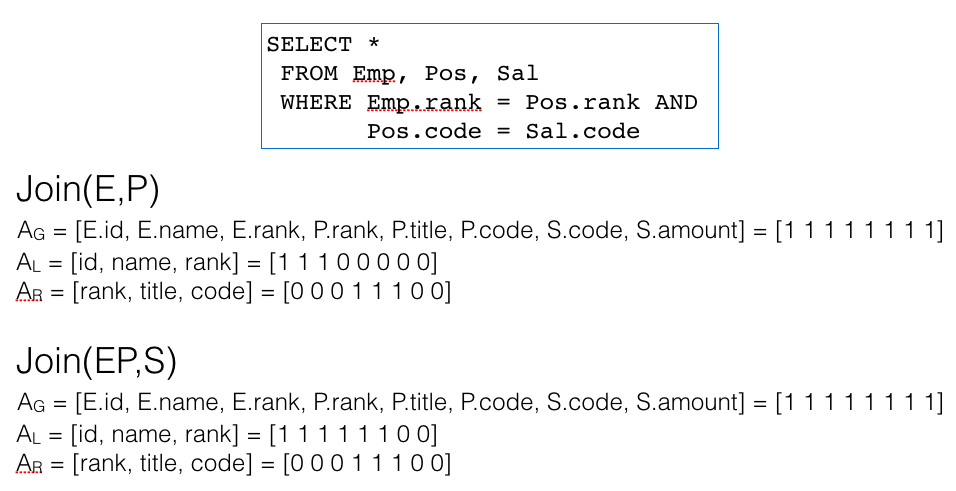
\includegraphics[width=0.7\textwidth]{figs/featurization.png}
    \caption{We use 1-hot encoding to capture which attributes participate in a join. This allows us to featurize both the query graph and the contraction. This figure shows the featurization for two different joins for the example query. \label{feat}}
\end{figure*}

To handle single relation selections in the query, we have to tweak the feature representation. This is because upstream selections and projections will change the cost properties of downstream joins. As in the classical optimizers, we eagerly apply selections and projections to each relation. 
Here, we leverage the table statistics present in most RDBMS. For each relation in the query graph, we can estimate a reduction factor $\delta_{r}$, which is an estimate of the fraction of tuples present after applying the selection to relation $r$. 
In the featurization described in the previous section, we have a set of binary features $V_{rel}$ that describe the participating attributes.
We multiply the reduction factors $\delta_r$ for each table with the features corresponding to attributes derived from that relation.
Figure \ref{feat:sel} illustrates the effect of adding a single table predicate to the example query. 

\begin{figure}
    \centering
    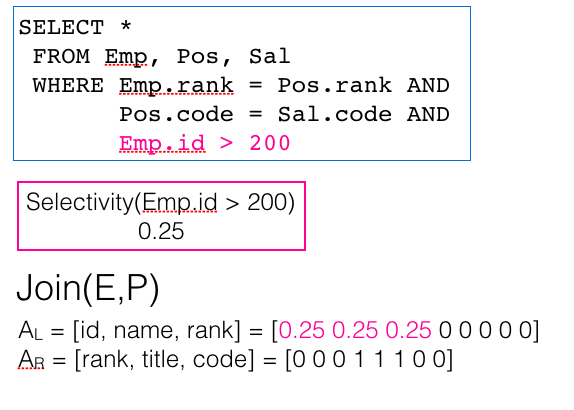
\includegraphics[width=\columnwidth]{figs/selectivity.png}
    \caption{To featurize single table selections, we scale the features by selectivity estimates given to use from a cost-estimator. \label{feat:sel}}
\end{figure}

\vspace{0.5em} \noindent \textbf{Join Condition: } The next piece is to featurize the join condition, or the predicate that defines the join. Participating relations define vertices and the predicate defines an edge. As before, let $A$ be the set of all attributes in the database. Each expression has two attributes and an operator. As with featurizing the vertices we can 1-hot encode the attributes present. We additionally have to 1-hot encode the binary operator $\{=,!=,<,>\}$. Concatenating all of these binary vectors together for each expression $\rho$ there there is a binary feature vector $f_\rho$.  For each of the expressions in the conjunctive predicate, we concatenate the binary feature vectors. Here is where the fixed size assumption is used. Since the maximum number of expressions in the conjunction capped at $\mathcal{N}$, we can get a fixed sized feature vector for all predicates. We call this feature vector $V_{cond}$ and it has dimensionality of $\mathcal{N} \cdot(|A|+4)$. 

\vspace{0.5em} \noindent \textbf{Representing the Q-Function: }
The Q-function is represented as a multi-layer perceptron (MLP) neural network.
It takes as input two feature vectors $V_{rel}$ and $V_{cond}$. Experimentally, we found that a two-layer MLP gave the best performance relative to the training time. We implmented the training algorithm in \textsf{DL4J} a java framework for model training with a standard DQN algorithm. The featurization approach is very extensible. Any property that we want the network to capture and be robust to can be added to the feature representation. For example, we can add an addition set of binary features $V_{ind}$ that indicate which attributes have indexes built on them. Handling, sort-orders are similar and we have to add features describing which attributes need to be finally sorted in the query. We can similarly add features that describe the available memory if we believe that is an important resource to manage in determining the final best plan.

\vspace{0.5em} \indent \textbf{Training: }

\[
\theta^{(i+1)} = \theta^{(i)} + \alpha \cdot [ (R + \max_{c'} Q_\theta(G',c')) - Q_\theta(G,c) ] \cdot \nabla Q_\theta(G,c) 
\]

\subsection{Generating the Training Data}
Experimentally, we found that the process of generating the process of training data for a given workload was very important for robust learning.
The basic challenge is that the Q-function must accurately be able to differentiate between good plans and bad plans.
If the training data only consisted of optimal plans, then the learned Q-function may not accurately score poor plans. Likewise, if the training purely sampled random plans--it may not see very many instances of good plans.
We want an efficient algorithm that avoids exhaustive enumeration to sample a variety of very good plans and poor plans.

The data generation algorithm, which we denote as \textsf{sample}$(G, \epsilon)$, takes as input a query graph $G$ and a randomization parameter $\epsilon \in [0,1]$.

\textsf{sample}$(G, \epsilon)$:
\begin{enumerate}
    \item \textbf{if} $\kappa_G = |G|$ return.
    \item For all graph contractions $c_i$ on G:.
    \begin{enumerate}
    \item $G_i = c_i(G)$  
    \item $V(c_i, G_i) = \textsf{leftDeep}(G_i)$
    \end{enumerate}
    \item \textbf{if} \textsf{rand()} $> \epsilon$: yield $c_j, G_j = \arg\max_{c_i} V(c_i,G_i)$, return \textsf{sample}$(G_j,\epsilon)$
    \item \textbf{else: } yield uniform random $c_j, G_j $, return \textsf{sample}$(G_j,\epsilon)$
\end{enumerate}

The algorithm essentially acts as the Q-Function algorithm described in the previous section. The algorithm proceeds as follows: (1) start with the query graph, (2) find the lowest cost contraction, (3) update the query graph and repeat. The lowest cost contraction is determined by assuming the remaining joins will be optimized with a left-deep strategy.
Let \textsf{leftDeep}(G) be the function that calculates the final cost of the best left deep plan given the query graph G.
To implement \textsf{leftDeep}(G), we use the System R dynamic program. 
This acts as an approximation to the Q function where the current step is locally optimal but future joins are efficiently approximate. {\reminder {Zongheng: I don't understand what ``efficiently approximate'' means. Do you mean ``efficiently approximated''?}}

To sample some number of poor plans in the training dataset, the $\epsilon$ parameter controls the number of randomly selected decisions.
This trades off reasonable optimality during training vs. covering the space of plans.
In this sense, we base the data generation algorithm in a particular \emph{workload}. The workload is a distribution over join queries that we want to optimize. 
We have an optimizer that samples some number of initial queries from the workload and is tested on unseen data.

\subsection{Execution after Training}
After training, we will have a parametrized estimate of the Q-function, $Q_\theta(f_G,f_c)$. For execution, we simply go back to the standard algorithm as in the greedy method but instead of using the local costs, we use the learned Q-function: (1) start with the query graph, (2) featurize each contraction (2) find the contraction with the lowest \textbf{estimated Q-value}, (3) update the query graph and repeat.

\section{Optimizer Architecture}
We call this new join optimization algorithm \sys, and describe how it fits into a query optimization stack. 

\subsection{API}
\sys optimizes Select-Project-Join (SPJ) blocks of SQL queries. To plug \sys into a query optimizer here are the API hooks that we require implemented:

\vspace{0.5em}
\begin{lstlisting}
sample(): List<Queries> 
\end{lstlisting}
\noindent A function that returns a list of training queries of interest.

\vspace{0.5em}
\begin{lstlisting}
train(query): List<Graph,Join,Graph',Cost> 
\end{lstlisting}
\noindent A function that given a query returns a list of join actions and their resultant costs. 

\vspace{0.5em}
\begin{lstlisting}
selectivity(predicate): Double
\end{lstlisting}
\noindent A function that returns the reduction factor of a particular single table predicate.

\vspace{0.5em}
Given these three functions, \sys can plug in to any system. It takes as input an SPJ block and outputs an optimized logical and physical join plan. 
Our prototype implementation is built on Apache Calcite.
The system connects to various database engines through a JDBC connector and has a internal simulator to model different physical design choices.

\subsection{Architectural Implications}
\textbf{TODO: Joe wanted to write something here}


\subsection{Limitations}
This work is meant to be an initial study of Deep Reinforcement Learning in the context of join optimization. There are a number of features expected of join optimizers that are not yet supported. We plan to add such support in future work but felt it was out of scope of this paper.

 \vspace{0.5em} \noindent \textbf{Sort Orders: } We do not consider cost models for sorting, sort-merge joins, or interesting orders. Keeping track of interesting sort orders in subplans is actually not difficult in our framework. They can be tracked as a set of additional features. 

\vspace{0.5em} \noindent  \textbf{Outer Joins/Inequality Joins: } We currently only consider optimization of inner joins and conjunctions of join conditions.


\section{Reduction factor learning}

Classical approaches to reduction factor estimation include (1) histograms and
heuristics-based analytical formulae, and (2) applying the predicate under
estimation to sampled data, among others.  In this section we explore the use of
learning in reduction factor estimation.  We train a neural network to learn the
underlying data distributions of a pre-generated database, and evaluate the
network on unseen, randomly selections that query the same database.

To gather training data, we randomly generate a database of several relations,
as well as random queries each consisting of one predicate of the form ``R.attr
$\langle$op$\rangle$ literal''.  For numeric columns, the operands are $\{=,
\neq, >, \geq, <, \leq\}$, whereas for string columns we restrict them to
equality and inequalities.  Each attribute's values are drawn from a weighted
Gaussian.

To featurize each selection, we similarly use 1-hot encodings of the participant
attribute and of the operand.  Numeric literals are then directly included in
the feature vector, whereas for strings, we embed ``hash(string\_literal) \% B''
where $B$ is a parameter controlling the number of hash buckets.  The labels are
the true reduction factors by executing the queries on the generated database.

A fully-connected neural network is used\footnote{Two hidden layers, 256 units
each, with ReLU activation.}, which is trained by stochastic gradient descent.

{\bf Evaluation.}  We compare the neural net to a simple linear regressor.  We
train on a database of 5 relations, a total of 21 attributes; the train and test
sets include 1000 and 2000 queries, respectively. We found that the fitted
linear regressor has a mean-squared-error of $\approx 84$, while the neural
network is able to achieve an L1 loss of $< 1$, approximating the true reduction
factors with minimal error.  \reminder {TODO(zongheng): they need to be on the
same scale. }

%\section{Search Overview}
We now provide an overview of \sys's search algorithm and optimizations.

% The optimization algorithm takes a quality function, a language, and a dirty relation, and outputs a sequence of transformations (of max depth $k$) that maximizes the quality function.

{
\begin{algorithm}[t]
\KwData{Q, R, $\Sigma$, $L$, (k, $\gamma$)}

// Initialize priority queue of candidate programs\\
$P = \{NOOP\}$

\While{ $|\{p \in P\ |\ p.len < k\}| > 0$ }
{
    \For{$p \in P: \|p\| < k$ }{
        
        Pop $p$ from the queue.
        
        \For{$T \in \Sigma$}{
             $p' = p \circ T$ 
             
             \If{$p' \in L$}{
               $P.push(p', Q(p'(R)))$
             }
        }
    }
    
    $\bar{p} = \argmax_{p\in P} Q(p(R))$\\
    $P = \{p \in P\ |\ p < \gamma\times Q(\bar{p}(R)) \}$
}

\Return Highest priority item on the queue
\caption{Greedy Best-First Tree Search}
\label{alg:main}
\end{algorithm}
}

\subsection{Naive Search Procedures}
In principle, any tree search algorithm over $L$ would be correct.
However, the traversal order and expansion policy is important in this search problem.  We describe the algorithmic and practical reasons why two naive procedures---breadth-first search (BFS) and depth-first search (DFS)---exhibit poor search runtimes.

\stitle{BFS} This approach extends each program in the search frontier with every possible data transformation in $\Sigma$.  To extend a candidate program $l_c$ with $T \in \Sigma$, it evaluates $Q((T\circ l_c)(R))$.  Unfortunately, the frontier grows exponentially with each iteration.  Additionally, evaluating every new candidate program $T\circ l_c$ can be expensive if the input relation is large.   Although the cost can be reduced by materializing $l_c(R)$, it is not possible to materialize all candidate programs in the frontier for all but the most trivial cleaning problems.    It is desirable to use asearch procedure that bounds the size of the frontier and the materialization costs.

% The first problem with this algorithm is that since each node in this tree $o$ represents a sequence of transformations.
% Evaluating the value of $o$ can be very expensive since it would have to evaluate the entire path to the root.
% $o$ is a composition of many transformations and may require a number of passes over the dataset.
% This can be avoided if we can materialize (either to disk or memory) the frontier,that is, for each node in the priority queue $o \in O$, we have a cached result of $o(R)$. 
% However, with BFS, the frontier is expoential in the support of the language and the system would quickly run out of memory.

\stitle{DFS} Depth-first search only needs to materialize the intermediate results for a single program at a time, however it is highly inefficient since the vast majority of programs that it explores will have low quality scores.  


\subsection{Search Algorithm and Optimizations}
Best-first search expands the most promising nodes chosen according to a specified cost function.
We consider a greedy version of this algorithm, which removes nodes on the frontier that are more than $\gamma$ times worse than the current best solution (\Cref{alg:main}).
Making $\gamma$ smaller makes the algorithm asympotically consistent but uses more memory to store the frontier, whereas $\gamma=1$ is a pure greedy search with minimal memory requirements.  

The frontier is modeled as a priority queue $P$ where the priority is the quality of the candidate program, and is initialized with a NOOP program with quality $Q(R)$.  
The algorithm iteratively extends all programs in the queue with less than $k$ transformations; a program $p$ is extended by composing it with a transformation $T$ in $\Sigma$.  If the resulting program $p'$ is in the language $L$, then we add it to the queue.
Finally, let $\bar{p}$ be the highest quality program in the queue.  The algorithm removes all programs whose quality is $<\gamma\times Q(\bar{p}(R))$ from the frontier.  
This process repeats until the candidate programs cannot be improved, or all programs have $k$ transformations.

In a naive and slow implementation, the above algorithm computes $p$'s quality by fully running $p$ on the input relation before running $Q$ on the result, explores all possible data transformation sequences, and runs sequentially.  One of the benefits of its simple structure is that it is amenable to a rich set of optimizations to prune the search space, incrementally compute quality functions, and parallelize the search.  In fact, we find that many optimizations in existing specialized cleaning systems can be cast in terms of the following classes.

% We can materialize (either to disk or memory) the frontier,that is, for each node in the priority queue $p \in P$, we have a cached result of $p(R)$. 
% Then, when we expand the nodes to $p' = p \circ t$, we only have to incrementally evaluate $t(R)$.
% After the node is expanded, the result is added to the cache if it within $\gamma$ of the best solution.
% The basic algorithm described above is well-suited for this problem.
% Without the greediness, the frontier might be exponentially large leading to an impractical amount of materialization.
% By tuning $\gamma$, the user can essentially set how much memory is used for materialization.


\btitle{Static Pruning Rules} are boolean functions that take a candidate program $p$ as input and decides whether it should be pruned. \sys currently models static rules as regular expressions over $\Sigma$.  Static rules are can be viewed as filters over $L$.
\[\textsf{static\_rule}(p) \mapsto \{0,1\}\]
For example, since the find-and-replace operations are idempotent, i.e., $T(T(R)) = T(R)$, we may want to only consider the set of all sequences with no neighboring repeated transformations. Similarly, we may also want to prune all search branches that make no effect (i.e., find-and-replace New York with New York).
These two regular expressions alone reduce the above example's language by $48\%$ (from 226981 to 120050).
Other rules, such as avoiding changes that undo previous changes $T^{-1}(T(R)) = R$, are similarly easy to add.


\btitle{Dynamic Pruning Rules} also have access to the input relation and quality function, and can make instance-specific pruning decisions.
\[\textsf{dyn\_rule}(p, Q, R) \mapsto \{0,1\}\]
For example, suppose  $Q$ is based on functional dependencies and is cell-separable, and we want to ensure that cell-level transformations made by a candidate program $p$ individually improve $Q$.  In this case, we find the cells $C$ that initially violate the functional dependencies and ensure that the cells transformed by $p$ are all in $C$.  Applying this optimization, in addition to the others in \sys, to the example reduces the search space by $143\times$ from 226,981 candidate programs to only 1582.  

Since it can be challenging to hand-write pruning rules, \Cref{s:dynlearn} describes a dynamic approach that uses simple machine learning models to automatically identify the characteristics of candidate programs to decide whether a particular search brach will be promising.  In essence, it generates and refines static pruning rules during the search process.  

%  it is a promising  and relation instance to decide whether the candidate program is promising to further explore.  In essense, it estimates the quality function of the search space rooted at $p$.

% For example, we may want to ensure that all the evaluations are ``correlated'' with the cost function--that is it makes modifications that are likely to affect the costs.  This is possible if the cost separable where we have a score for each cell. In this case, we can find all the cells in violation of the functional dependencies and make sure that the ``source'' field of the find-and-replace operations only match values that are in violation.  These optimizations are called ``dynamic' because they can be determined from the active domain (i.e., after applying a transformation, recalculate new optimization rules).  Applying this optimization (in addition to the others) to the example reduces the search space to 1582 evaluations v.s. 226981 unoptimized (143x reduction).

\stitle{Block-wise Cleaning} 
A major cost is that independent errors in the relation must be cleaned sequentially in the search algorithm.  For instance, records 2, 3, and 4 in~\Cref{ex1} exhibit independent errors and a fix for a given record does not affect the other records.  Thus, if each record were cleaned in isolation, the search space would be $O(|\Sigma|)$.  Unfortunately, the entire relation requires a program of three transformation to fix the records, which increases the search space to $O(|\Sigma|^3)$.

The main insight in block-wise cleaning is that many errors are local to a small number of records.  In these cases, it is possible to partition $R$ into a set of blocks $B_1,\cdots,B_m$, execute the search algorithm over each block independently, and concatenate their programs to generate the final cleaning program.  This gather-scatter approach can exponentially reduce the search space for each block, and reduces the cost of evaluating super-linear quality functions that require e.g., computing a pair-wise similarity scores for the input relation.    For example, quality functions derived from functional dependencies can define blocks by examining the violating tuples linked through the dependency.  Similarly, users can define custom partitioning functions or learn them via e.g., clustering algorithms.  In our current implementation, we partition the input relation by cell or row if the quality function is cell or row separable.


% so makes >linear pruning costs faster
% and if cleaning xforms are independent
% There are two types of paraellization.  row-wise by gather scattering over the blocks, and evaluating candidate programs in parallel.  We support both.  It's particularly easy for decomposable quality and xforms.
% the whole dataset might require 15 transforms to clean
% but only 1 transform per block
% 
% so makes >linear pruning costs faster
% and if cleaning xforms are independent


\stitle{Parallel Program Evaluation} It is clear that the candidate programs can be evaluated and pruning in a parallel fashion across multiple cores and multiple machines, and is one of the major innovations in modern planning systems.  However, unlike classic planning problems where communications are small due to the compact size of each state, \sys's state size is determined by the relation instance, and can lead to prohibitively high communication costs and memory caching requirements.   Section~\ref{s:parallel} describes how we manage the trade-offs when parallelizing \sys in shared memory and distributed settings.

\stitle{Materialization} Since each candidate program $p' = p\circ T$ is the composition of a previous candidate program and a transformation, an obvious optimization is to materialize the output of $p(R)$ and incrementally compute $p'(R)$ as $T(p(R))$ over the materialized intermediate relation.  Although this works well in a single threaded setting, memory and communication challenges arise when combining materialization with parallelization (\Cref{s:parallel}).

% Arbitrary constraint satisfaction problems are challenging because all variables can interact. While this is certainly the case for arbitrary quality functions, in many cases, data errors are localized. For example, replacing \texttt{San Francisc} with \texttt{San Francisco} has no effect on the records referring to \texttt{New York City}. The final class of optimizations are blocking rules which have been widely used in entity resolution systems:
% \[\textsf{block}(Q, R, L) \mapsto \{R_1,...,R_k\} \]
% For quality functions generated from dependencies, we can determine blocks analytically--looking at which violating tuples are linked through the constraint.
% However, in general, these blocking rules can be learned (e.g., with clustering) or user defined.
% The search can execute on each of the blocks independently.
% \ewu{Emphasize that this is based on the decomposable nature of the quality function}

% \stitle{Quality Estimation}  A large cost to the search algorithm stems from the need to execute the quality function over the output of each candidate program.  In some cases, it is possible to estimate the quality function without fully running the candidate program.  For instance, \ewu{foofah}.  Alternatively, it may be sufficient to run the candidate program over a sample of the input relation.  These are opportunities for future work.  \textbf{TODO}





%\begin{figure}[t]
    \centering
    \includegraphics[width=\columnwidth]{figures/distributed.pdf}
    \caption{In each iteration, each worker starts with a subset of the priority queue (boxes).  The driver sends a subset of data transformations from $\Sigma$ (circles) to generate candidate programs (box-circles).  A series of synchronization points identify the globally top $\gamma$ candidates and redistributes them across the workers.   \label{fig:algo}}
\end{figure}

\section{Search Optimizations}\label{s:opts}
This section describes two important optimizations that allows \sys to generate cleaning programs in comparable runtimes as specialized systems.

\subsection{Parallelization}\label{s:parallel}
Composing and evaluating $Q(p'(R))$ is the single most expensive operation in the search procedure.   We now discuss how we parallelize its evaluation in shared memory and distributed settings, and the challenges when combining it with materialization.

\stitle{Shared Memory} In a naive, shared-memory implementation, we execute all expansions for a given $p\in P$ in parallel.  We materialize $p(R)$ in memory, and evaluate the quality of each $p' = p\circ T\ |\ T \in \Sigma$ in parallel using a  thread pool.  Each thread drops a given $p'$ if its quality is lower than $\gamma\times$ the maximum quality from the previous \texttt{WHILE} iteration or the local thread.  At the end of the \texttt{WHILE} iteration, the threads synchronize to compute the highest quality, and flush the remaining candidates using the up-to-date quality value.  The output of each $p'(R)$ can be retained or discarded using any cache replacement policy.  Our implementation uses Ray~\cite{ray} to schedule and parallelize the tasks.

\stitle{Distributed}
In the distributed setting, we do not have access to fast shared memory and the communication costs of sharing intermediate relations $p(R)$ can be impractical.  Thus, each worker is given a subset of candidate programs to locally evaluate and prune, and the main challenge is to reduce task skew through periodic rebalancing.  We use a worker-driver model with $j$ workers (\Cref{fig:algo}).

Let $P^{next} = P\times \Sigma$ be the set of candidate programs (e.g., \includegraphics[height=8pt]{figures/program.pdf}) to evaluate in the current iteration of the search algorithm. For instance, $P=\{NOOP\}$ in the first iteration, so the candidates are the set of individual data transformations $\Sigma$.   The driver assigns the input relation $R$ and $\frac{1}{j}$ of $P^{next}$ to each worker.  In the figure, the driver assigns a subset of $\Sigma$ to each worker.  Each worker evaluates and computes the top-$\gamma$ candidates based on the best worker-local quality.   The worker runs and caches the parents of its assigned candidate programs (\includegraphics[height=8pt]{figures/sq-blue.pdf}, \includegraphics[height=8pt]{figures/sq-grey.pdf}) to incrementally compute the quality function.
  
Note that the worker-local top-$\gamma$ candidates are a superset of the top-$\gamma$ global candidates because the best local quality is $\le$ the global best.   Thus the workers synchronize with the driver to identify the global best candidate and further prune each worker's top candidates.  At this point, all candidate programs are within $\gamma$ of the globally best candidate, but their distribution across the workers can be highly skewed.  \sys performs a final rebalancing step, where each worker sends the number of un-pruned candidates to the driver.  Workers with more than $\frac{1}{j}$ of the total number redistribute the extras to workers with too few candidates.  When redistributing, workers communicate directly and do not involve the driver (e.g., Worker 2 sends \includegraphics[height=8pt]{figures/program-greyred.pdf} to Worker 1).   If the total number is $<k$, then candidates are randomly chosen to be replicated.  Only the programs and their qualities are sent; the program results are re-computed by the receiving worker.  This ensures that the priority queue in the next iteration is evenly distributed across all workers.  

% The workers then communicate the quality of their best transformation. This can be used to reconcile the local materializations to only the global top-$\gamma$ set.  This set is not necessarily balanced, e.g., one worker might have almost all of the top transformations.  The next step is a balancing step, where each worker communicates the number of materialized expansions it currently stores.  The workers with more than $\frac{|O|}{j}$ materialized expansions  randomly select ones to evict, and the driver re-distributes these to nodes with too few materialized expansions.  This is done by communicated the transformation and the result is re-computed on the new worker.  If $|O| < k$, then expansions are chosen at random to be replicated.  The result of the reconciliation step is that all workers have an evenly distributed set of materialized expansions.

% \item \ititle{Next Round} After reconciliation, each worker is associated with a particular $o \in O$ (or a set of them). To parallelize, the driver must simply ensure that it assigns new expansions only to those workers that have materialized the parent.  The algorithm then repeats, expanding each node locally, and then reconciles the results.

% The best-first search algorithm also is amenable to parallelization. One can parallelize over the two inner for loops $O \times L$. Each expansion can be forked into its own thread. However, this actually makes the materialization described above a bit more challenging. We use Ray~\footnote{https://github.com/ray-project/ray} to implement the parallel search. 
% 
% \subsubsection{Shared Memory Parallelization}
% The most straight-forward case is when we have access to low-latency shared memory between the expansion threads. In each expansion round, the main thread will assign each expansion node to workers and they will evaluate a given transformation. Each worker will make a copy of $o(R)$ (the node it is expanding) into shared memory. 
% If the expanded transformation is within $\gamma$ of the best current result, then it will update the copy, otherwise delete it. 
% 







\subsection{Dynamically Learning Pruning Rules}\label{s:dynlearn}
To effectively search through the language of transformations, pruning heuristics are important, yet hand-writing such heuristics {\it a priori} is challenging.
We describe how such heuristics can be automatically learned during the cleaning process.

\stitle{Motivation}
The search algorithms in  most automatic data cleaning frameworks are carefully tuned for a specific quality function or class of quality functions. For example, the chase used in functional dependency resolution does not make an edit to the table unless it enforces at least one tuple's FD relationship.    Similarly, in entity matching problems, one restricts the search to only matching tuples that are likely to be similar based on some similarity metric.
These can be viewed as search pre-conditions that exploit the structure of the cleaning problem to a more tractable search space.
Note that these are not static optimizations: knowing how to prune the search space requires identifying and modeling the structure of the underlying data errors and how they interact with the data transformations.
% the underlying data or making strong modeling assumptions about the types of transformations used.

%\ewu{So you're not training based on how the quality function changes as a program gets longer?  If each training example is simply the program for a block, how many blocks does there need to be?  If the search process isn't doing a great job, does that mean the learned classifier will suck?}

\stitle{Approach}
When \sys executes the search algorithm on each block of data, it generates a cleaning program that optimizes the quality metric for that block.  In many cases, the dataset can be partitioned into a large number of blocks that each serve as sources of training examples for a learned pruning model.  Each transformation in a block's  cleaning program $p_b$ can be labeled as a positive training example in $\Sigma_b^+$, while all other transformations serve as negative examples $\Sigma_b^- = \Sigma - \Sigma_b^+$.
As \sys processes more blocks, the union of these training sets can be sufficient to train a classifier to predict whether a given transformation will be included in the optimal program.  In our approach, the prediction model $M(T): \Sigma \mapsto \{0,1\}$ is over the data transformations and not the data; is this sense, \sys learns static pruning rules in a dynamic fashion.    

% \sys executes the search on each block of data.  The result is a sequence of transformations to optimize the quality metric on that block.  Every transformation in this sequence can be treated as a positive training example $L^+$, and every transformation not in this sequence can be treated as a negative example $L^-$.  The idea is that if we apply the search to a sufficient number of blocks then we can train a classifier to predict whether a transformation will be included in the final sequence.  It is important to note that this prediction is over the transformations and not the data. 

Internally, \sys uses a Logistic Regression classifier that is biased towards false positives (i.e., keeping a bad search branch) over false negatives (e.g., pruning a good branch). This is done by training the model and shifting the prediction threshold until there are no False Negatives. 


\stitle{Featurization}
To use this approach, we use featurizers to transform each data transformation $T$ into a $k$-dimensional feature vector: \textsf{feat}: $T\mapsto\mathbb{R}^k$.
For example, recall the \texttt{find\_replace(NYC, NY, city\_code)} transformation in~\Cref{ex1}.
The expert is free to encode potential signals as part of the transformation.  For instance, the edit distance between the two literal parameters (e.g., NYC, NY) and an indicator vector to specify the attrbitue (e.g., city\_code).  

Notice that many data transformation can be modeled as a predicate that specifies which records to clean, target attributes to clean, and replacement values for those attributes.  Thus, the featurized transformation potentially allows a model to learn which records, which attributes, and what replacement values, are highly to contribute to the final cleaning program.  For instance, \sys may learn that \texttt{find\_replace} only makes sense for \texttt{city\_name}.  Similarly, it may learn that the replacement string should be similar in edit distance to the source string, and subsequently learn the appropriate edit distance threshould.


\stitle{Discussion} We believe this is one of the reasons why a simple best-first search strategy can be effective.  For the initial blocks, \sys searches without a learned pruning rule in order to gather evidence.  Over time, the classifier can identify systematic patterns that are unlikely to lead to the final cleaning program, and explore the rest of the space.  In fact, this incremental learning process can be viewed from an active learning perspective to further target the exploration towards programs that will best improve the classification model.  

A potential benefit of learning a pruning model for {\it data transformations} rather than relation instances is that it can potentially be reused or fine-tuned for new, but structurally similar, data cleaning problems. In this way, the model can be trained {\it across data cleaning problems} rather than across blocks within a single problem.    In addition, we speculate that across a sufficient number of cleaning problems, if they share a common set of data transformation, we may adapt a deep learning approach to automatically learn the features themselves.  


% For example, some columns might not be dirty and are not worthwile to clean.  In the example above, another observation could be that the source and target strings in the optimal sequence are very close in terms of string similarity (as opposed to arbitrary transformations).  If each of these operations was featurized with a single scalar that is the edit-distance between the two strings, then the classifier could learn a pruning threshold (i.e., not considering find-and-replace operations above that threshold).  

% Consider an alternative to a predefined search heuristic where we clean data in small blocks.  For the initial blocks, we search without a heuristic.  As we continuously perform the search, we train a classifier on these features to reject search branches that are not typically in the final solution.  This allows us to exploit any patterns in the literal parameters that repeatedly occur.




%\section{Experiments}
Leis et al. recently argued for improved benchmarks for evaluating join ordering algorithms, and proposed the ``Join Order Benchmark'' (JOB)~\cite{leis2015good}.
This benchmark is derived from the Internet Movie Data Base
(IMDB). It contains information
about movies and related facts about actors, directors,
production companies, etc. 
The dataset is 3.6 GB large and consists of 21 relational tables.
The largest table has
36 M rows.
The benchmark contains 33 queries which have between 3 and 16 joins, with an average of 8 joins per query. 
We evaluate \sys on this benchmark in terms of planning latency and plan cost.


\subsection{JOB Cost Models}
As a secondary contribution of this paper, we find that the particular choice of cost model and physical design greatly affects results.
The same query with different cost models can lead to different top-performing heuristics.
Crucially, we find that many heuristics are sensitive to non-linearities.

The cost model described in~\cite{leis2015good} is inspired by an in-memory system. The cost of a hash join is linear in the size of the input relations, and the cost of a index join is essentially the cost of streaming the left side of the join.
This cost model greatly rewards index-usage (by convention the right relation is used for index lookup), and left-deep strategies are very strong in this setting. In fact, the authors quote: 
\begin{quote}
\emph{``The bad performance of right-deep trees is caused by the large intermediate hash tables that need to be created from each base relation and the fact that only the bottom-most join can
be done via index lookup.''}~\cite{leis2015good} 
\end{quote}
The conclusion is that the marginal benefit of bushy plans is small compared to the additional search costs.
We argue that this is a consequence of the cost model and physical design and this led us to explore alternative cost models where the left-deep heuristic might fail.

\vspace{0.25em} \noindent \textbf{CM1: } In the first cost model (inspired by~\cite{leis2015good}), we model a main-memory database that performs two types of joins: index nested-loop joins and in-memory hash joins. Let $O_l$ be the left operator and $O_r$ be the right operator the costs are defined as follows:
\[
\textsf{c}_{inlj} = \textsf{c}(O_l) + \textsf{rf}(O_l, O_r) \cdot |O_l|
\]
\[
\textsf{c}_{hj} = \textsf{c}(O_l) + \textsf{c}(O_r)
\]
where \textsf{c} denotes the cost estimation function and \textsf{rf} denotes the estimated reduction factor of the join.
As we can see, this model favors index-based joins when available. 
The reduction factor $\textsf{rf}(O_l, O_r)$ is always less than 1.
More importantly, this cost model is a justification for the use of left-deep plans.
In $\textsf{c}_{inlj}$, the right operator does not incur a scan cost.
A left deep tree where the indexed relations are on the right exploits this structure. We include primary key and foreign indexes on all relations.


\vspace{0.25em} \noindent \textbf{CM2: } In the next cost model, we model a database that accounts for disk-memory relationships in the hash joins. We designate the left operator as the ``build'' operator and the right operator as the ``probe'' operator. 
If the previous join has already built a hash table on an attribute of interest, then the hash join does not incur another cost.
\[
\textsf{c}_{nobuild} = \textsf{c}(O_r)
\]
This model favors right-deep plans where to maximize the reuse of the built hash tables.


\vspace{0.25em} \noindent \textbf{CM3: } Finally, in the next cost model, we model temporary tables and memory capacity constraints. There is a budget of tuples that can fit in memory and an additional physical operator that allows for materialization of a join result if memory exists. Then, the downstream cost of reading from a materialized operator is 0.   
\[
\textsf{c}(O) = 0 \text{ if materialized}
\]
This model requires bushy plans due to the inherent non-linearity of the cost function and memory constraints. 
The cost model encourages plans that group tables together in ways that the join output can fit in the available memory.

\vspace{0.5em} In our implementation of these cost models, we use \emph{true} cardinalities on single table predicates and two-way joins of base relations. We leverage standard independence assumptions to construct more complicated cardinality estimates. The goal of this work is to evaluate the join ordering process independent of the strength or weakness of the underlying cardinality estimation. 

\subsection{Baseline Algorithms}
We consider the following baseline algorithms. These algorithms are not meant to be a comprehensive list of heuristics but rather representative of a class of solutions.

\begin{enumerate}
    \item Exhaustive (\textbf{EX}): This is a dynamic program that exhaustively enumerates all join plans avoiding cartesian products.
    \item Left-Deep (\textbf{LD}): This is a dynamic program that exhaustively enumerates all left-deep join plans.
    \item Right-Deep (\textbf{RD}): This is a dynamic program that exhaustively enumerates all right-deep join plans.
    \item Zig-Zag (\textbf{ZZ}): This is a dynamic program that exhaustively enumerates all zig-zag trees that is every join has at least one base relation (either on the left or the right).
    \item IK-KBZ (\textbf{KBZ}): This algorithm is a polynomial time approximation that decomposes the query graph into chains and orders the chains based on a linear approximation.
    \item QuickPick-1000 (\textbf{QP}): This algorithm randomly selects 1000 joins and returns the best of them. 1000 was selected to be roughly equivalent to the planning latency of \sys.
\end{enumerate}

\subsection{Optimizer Cost}
In the first experiment, we evaluate all of the baseline algorithms against \sys in terms of final optimization cost. All of the algorithms consider join ordering without cartesian products, so \textbf{EX} is a baseline optimal solution. We report results in terms of the suboptimality w.r.t \textbf{EX}.

\subsubsection{Without Single Table Selections}
We first evaluate consider the 33 join order benchmark query templates without single table selections. We train on 26 queries and test on 7 held out queries. We report results averaged over 5-fold cross-validation (so all of the reported numbers are when the query is not seen during training). We report the min, mean, and max cost relative to the baseline.  For randomized algorithms the max range of performance (as a multiplicative factor) over 5 trials.

In the first experiment, we consider CM1. This is an idealized model that heavily encourages index usage. All of the optimal plans for this workload are left-deep. Predictably, right-deep plans perform very poorly. \sys significantly out performs the heuristic solutions \textbf{KBZ} and \textbf{QP}. \sys is also far more reliable in terms worst case performance. 

\begin{table}[ht!]\centering \small
\caption{CM1 No Selections. Cost Relative to Optimal Plan. }\vspace{0.25em}
\begin{tabular}{|l|l|l|l|l|}
\hline
    & {\bf Min}  & {\bf Mean}  & {\bf Max}    & {\bf Range-Max} \\ \hline
{\bf QP}  & 1.0  & 23.87 & 405.04 & 2.11x      \\ \hline
{\bf KBZ} & 1.0  & 3.45  & 36.78  & -         \\ \hline
{\bf RD}  & 4.70 & 53.25 & 683.35 & -         \\ \hline
{\bf LD}  & 1.0  & 1.0   & 1.0    &           \\ \hline
{\bf ZZ}  & 1.0  & 1.0   & 1.0    & -         \\ \hline
{\bf EX}  & 1.0  & 1.0   & 1.0    & -         \\ \hline
\hline
{\bf DQ}  & 1.0  & 1.36   & 3.11    & 1.79x\\ \hline
\end{tabular}
\end{table}

By simply changing the cost model, we can force exactly the opposite heuristic to perform well. When we evaluate CM2, which accounts for reuse of hash tables, right-deep plans are no longer so poor. In this cost model, none of the heuristics match the exhaustive search over the entire workload. \sys comes close and it is actually significantly better than zig-zag enumeration for this cost model.

\begin{table}[ht!]\centering \small
\caption{CM2 No Selections. Cost Relative to Optimal Plan. }\vspace{0.25em}
\begin{tabular}{|l|l|l|l|l|}
\hline
    & {\bf Min}  & {\bf Mean}  & {\bf Max}    & {\bf Range-Max} \\ \hline
{\bf QP}  & 1.43  & 16.74 & 211.13 & 1.71x      \\ \hline
{\bf KBZ} & 2.21  & 14.61  & 96.14  & -         \\ \hline
{\bf RD}  & 1.83 & 4.25 & 69.15 & -         \\ \hline
{\bf LD}  & 1.35  & 5.21   & 55.45    &           \\ \hline
{\bf ZZ}  & 1.0  & 3.41   & 23.13    & -         \\ \hline
{\bf EX}  & 1.0  & 1.0   & 1.0    & -         \\ \hline
\hline
{\bf DQ}  & 1.0  & 1.91   & 13.14    & 1.43x\\ \hline
\end{tabular}
\end{table}

CM3 is meant to illustrate a cost-model where no heuristic performs well. We count the number of tuples materialized and to benfit from the materialization these tuples must fit into memory. This leads to a ``packing'' like optimization problem where the exact join order also depends on how well the intermediate results can be packed into memory. \sys is still performant in this setting as it adapts to the properties of the workload.

\begin{table}[ht!]\centering \small
\caption{CM3 No Selections. Cost Relative to Optimal Plan. }\vspace{0.25em}
\begin{tabular}{|l|l|l|l|l|}
\hline
    & {\bf Min}  & {\bf Mean}  & {\bf Max}    & {\bf Range-Max} \\ \hline
{\bf QP}  & 1.78  & 46.19 & 489.13 & 3.44x      \\ \hline
{\bf KBZ} & 1.21  & 56.44  & 296.14  & -         \\ \hline
{\bf RD}  & 4.41 & 87.25 & 369.97 & -         \\ \hline
{\bf LD}  & 1.21  & 49.32   & 255.60    &           \\ \hline
{\bf ZZ}  & 1.16  & 21.44   & 243.16    & -         \\ \hline
{\bf EX}  & 1.0  & 1.0   & 1.0    & -         \\ \hline
\hline
{\bf DQ}  & 1.0  & 3.76   & 113.89    & 2.51x\\ \hline
\end{tabular}
\end{table}

\vspace{0.5em}\noindent \textbf{Summary and Caveats: }  We showed that heuristics are often myopic and can perform very poorly when the problem structure changes. A learning-based approach can adapt to the different scenarios at the cost of training data. As a caveat, we used idealized cost models with true cardinality values to evaluate the performance of different optimization and pruning heuristics. The experiment is meant to illustrate the mathematical structure of the optimization problem and does not make a claim about execution performance or plan variance.

\subsubsection{With Single Table Selections}
Next, we show the performance of \sys on the 113 JOB queries when we include single table selections. The point of this experiment is to illustrate an interesting difference between learning-based and enumeration-based optimization. When true cardinalities are available, single table selections are not a problem for classical optimizers, but a learning optimizer has to correlate reduction factors with changes in join decisions. This is difficult without observing a lot of different predicates at a variety of selectivities.
It is easy to generate a large dataset with a lot of different join orders, however, generating random predicates on the tables can be more challenging. We train on 80 queries and test on 33 queries. We do 4 fold cross validation to ensure that every test query is excluded from the training set at least once. 

\begin{table}[ht!]\centering \small
\caption{Effect of Single Table Selections on \sys }\vspace{0.25em}
\begin{tabular}{|l|l|l|l|l|}\hline
    & {\bf Min}  & {\bf Mean}  & {\bf Max}    & {\bf Range-Max} \\ \hline
{\bf CM1. No Sel}  & 1.0  & 1.36   & 3.11    & 1.79x\\ \hline
{\bf CM1. Sel}  & 1.0  & 2.14   & 8.43    & 2.86x\\ \hline
{\bf CM2. No Sel}  & 1.0  & 1.91   & 13.14    & 1.43x\\ \hline
{\bf CM2. Sel}  & 1.0  & 3.55   & 38.54    & 1.96x\\ \hline
{\bf CM3. No Sel}  & 1.0  & 3.76   & 113.89    & 2.51x\\ \hline
{\bf CM3. Sel}  & 1.0  & 6.44   & 207.09    & 3.56x\\ \hline
\end{tabular}
\end{table}

One approach addressing this issue is to augment the dataset with synthetic predicates. We could randomly sample equality conditions on each of the single tables. Figure \ref{exp:plot1} illustrates the results. We augment our training workload with a 100 additional training queries with random single table selections. With this data, we can better attribute the effects of selection on costs.   

\begin{figure}
    \centering
    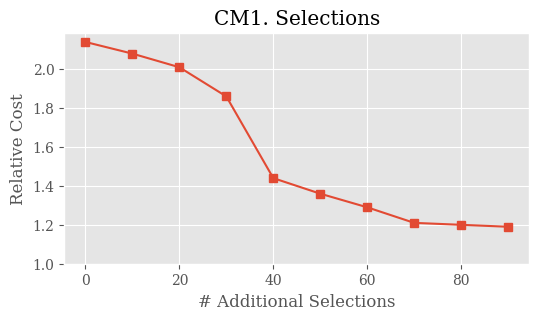
\includegraphics[width=0.8\columnwidth]{exp/exp1_plot1.png}
    \caption{Accurately modeling the effects of single table selections requires more training data. Generating a modest number of synthetic single table equality predicates can help. \label{exp:plot1}}
\end{figure}

Selections are interesting because they have threshold effects on cost. Once a selectivity of a predicate on one of the relations drops beyond a certain point--the set of low cost plans might drastically change. These results are both positive and negative. First, it illustrates that learning-based approaches can easily be made robust to different phenomena by manipulating the training data and/or the featurization. On the other hand, the system may not accurately be able to assess its own confidence on previously unseen plans. It might make predictions assuming smooth behavior without knowledge of a drastic change due to selectivity. 

\subsection{Data Quantity/Quality}
We further evaluate the nature of training data required by \sys, in terms of raw quantity (number of training queries seen) and quality (the relevance to the test workload).

\subsubsection{Quantity}


\subsubsection{Model-Limited or Data-Limited}
In theory, with enough data, \sys should be approaching optimal performance.
The natural next question is where does the gap come from---is it the neural networks ability to represent the cost function (Model-Limited) or is it a lack of training data (Data-Limited).
We ran an experiment on the first 20 training queries. \sys sees these queries in training as well as during testing. This measures the ability to memorize training data.






%\section{Related Work and Alternative Architectures}
Applications of machine learning in database internals is still the subject of significant debate this year and will continue to be a contentious question for years to come~\cite{btree, kraska2018case, mitzenmacher2018model, ma2018query}. An important question is what problems are amenable to machine learning and AI solutions. We believe that query optimization is one such sub-area. The problems considered are generally hard and orders of magnitude of performance are at stake. In this setting, correctness is not concern as poor learning solutions will lead to slow but not incorrect execution.

\subsection{Cost Function Learning} 
Admittedly, we are not the first to consider ``learning'' in the query optimizer and there are a number of alternative architectures that one may consider. The precursors to this work are attempts to correct query optimizers through execution feedback.
One of the seminal works in this area is the LEO optimizer~\cite{markl2003leo}. This optimizer uses feedback from the execution of queries to correct inaccuracies in its cost model. The underlying cost model is based on histograms. The basic idea inspired several other important works such as~\cite{chaudhuri2008pay}. The sentiment in this research still holds true today; when Leis et al. extensively evaluated the efficacy of different query optimization strategies they noted that feedback and cost estimation errors are still challenges in query optimizers~\cite{leis2015good}. A natural first place to include machine learning would be what we call \emph{Cost Function Learning}, where statistical learning techniques are used to correct or replace existing cost models. This is very related to the problem of performance estimation of queries~\cite{akdere2012learning, wu2013predicting, wu2013towards}. 

We actually started with this model, where a neural network learns to predict the selectivity of a single relation predicate. Results were successful, albeit very expensive from a data perspective. To estimate selectivity on an attribute with 10k distinct values, the training sets had to include 1000 queries. This architecture suffers from the problem of \emph{featurization of literals}; the results are heavily dependent on learning structure in literal values from the database that are not always straightforward to featurize. This can be especially challenging for string or other non-numerical data types.  A recent workshop does show some promising results in using Deep RL to construct a good feature representation of subqueries but it still requires $>$ 10k queries to train~\cite{ortiz2018learning}. 

\subsection{Adaptive Query Optimization}
Adaptive query processing is another line of work that we might think is relevant to the discussion~\cite{avnur2000eddies,deshpande2007adaptive} and the related techniques to re-optimize queries during execution~\cite{markl2004robust, babu2005proactive}. Reinforcement Learning studies sequential problems and adaptive query optimization is naturally a sequential decision problem.
We focus our study on optimization in fixed databases and the adaptivity that we offer is at a workload level. Continuously updating a neural network can be challenging for very fine-grained adaptivity for processing different tuples in different ways. 

\subsection{Join Optimization At Scale} 
Scaling up join optimization has been an important problem for several decades, most recently~\cite{neumann2018adaptive}. 

\textbf{TODO}







 



%\section{Conclusion and Future Work}

%NSF 1527765, 1564049.
Jiannan







%\bibliographystyle{abbrv}

{
%\fontsize{8.8pt}{9.7pt} \selectfont
\small
\bibliographystyle{abbrv}
\bibliography{ref} 
\scriptsize
}


%\appendix
\label{s:appendix}

\section{Quality Functions}
Details about quality functions for exsiting stuff

\section{Data Transformations}

Details about data xforms that we used.

\section{Datasets}
\vspace{0.5em}\noindent\textbf{USCensus: } This dataset contains US Census records for adults and the goal is to predict  whether the adult earns more than $50,000$ dollars. It contains 32,561 records with 15 numerical and categorical attributes. This dataset contained missing values and coding inconsistencies.
Examples of data error include:
\begin{lstlisting}
#missing values
40,Private,121772,Assoc-voc,11,
Married-civ-spouse,Craft-repair,Husband, 
Asian-Pac-Islander,Male,0,0,40,(*\orange{\bf{?}}*),>50K

#coding inconsistency
57,Local-gov,110417,HS-grad,9,
Married-civ-spouse,Craft-repair,Husband,
White,Male,(*\orange{\bf{99999}}*),0,40,United-States,>50K
\end{lstlisting}


\vspace{0.5em}\noindent\textbf{Federal Election Commission Contributions: } The FEC provides a dataset of election contributions of 6,410,678 records with 18 numerical, categorical and string valued attributes. This dataset has a number of errors. There are missing values, formatting issues (where records have the wrong number of fields causing misaligment in parsing), and numerical outliers (negative contributions).

\begin{lstlisting}
#missing values
C00458844,"P60006723","Rubio, Marco","RUCINSKI,
ROBERT","APO","AE","090960009","US ARMY",
"PHYSICIAN",100,08-MAR-16,(*\orange{\bf{``''}}*),(*\orange{\bf{``''}}*),(*\orange{\bf{``''}}*),"SA17A",
"1082559","SA17.1074981","P2016"

#rejected contributions double recorded
C00458844,"P60006723","Rubio, Marco","SWAID, 
SWAID N. DR.","BIRMINGHAM","AL","352660827",
"NEWOLOGICAL SURGERY ASSOCIATES","PHYSICIAN",
(*\orange{\bf{-400}}*),28-DEC-15, "REDESIGNATION TO GENERAL","X",
"REDESIGNATION TO GENERAL","SA17A",
"1047126","SA17.892835B","P2016"
\end{lstlisting}


\end{document}
